\hypertarget{_sb_integral_8c}{
\section{/home/mgh/LanlGeoMag/libLanlGeoMag/SbIntegral.c File Reference}
\label{_sb_integral_8c}\index{/home/mgh/LanlGeoMag/libLanlGeoMag/SbIntegral.c@{/home/mgh/LanlGeoMag/libLanlGeoMag/SbIntegral.c}}
}
{\tt \#include \char`\"{}Lgm/Lgm\_\-MagModelInfo.h\char`\"{}}\par


Include dependency graph for SbIntegral.c:\nopagebreak
\begin{figure}[H]
\begin{center}
\leavevmode
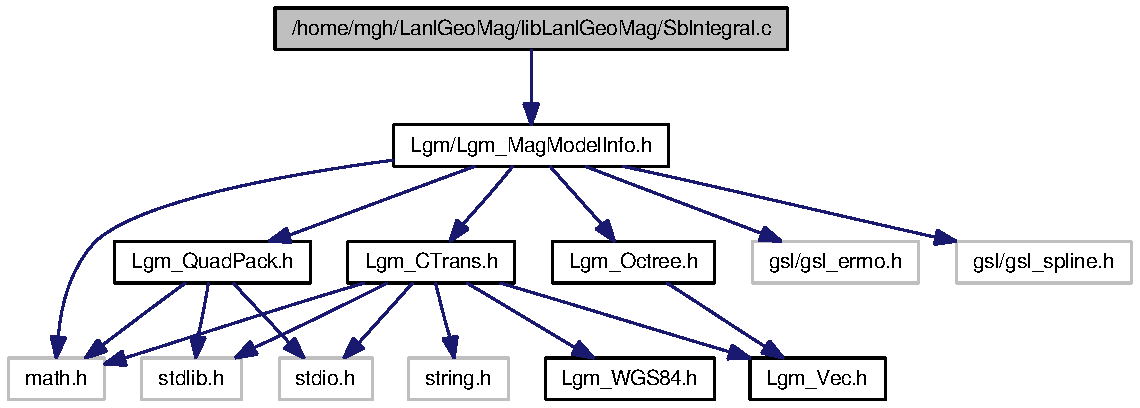
\includegraphics[width=291pt]{_sb_integral_8c__incl}
\end{center}
\end{figure}
\subsection*{Defines}
\begin{CompactItemize}
\item 
\#define \hyperlink{_sb_integral_8c_478cd83265b9c9a6b181dab783cb6fb8}{JUMP\_\-METHOD}~1
\end{CompactItemize}
\subsection*{Functions}
\begin{CompactItemize}
\item 
double \hyperlink{_sb_integral_8c_64cd517218ca183a56b43dfc1cf7b124}{SbIntegral} (\hyperlink{struct_lgm___mag_model_info}{Lgm\_\-MagModelInfo} $\ast$fInfo)
\item 
double \hyperlink{_sb_integral_8c_d53ba64293ea16f5d1878d483d62fcd4}{SbIntegral\_\-interped} (\hyperlink{struct_lgm___mag_model_info}{Lgm\_\-MagModelInfo} $\ast$fInfo)
\item 
double \hyperlink{_sb_integral_8c_1828b0051c3925909496a0d956bcaab3}{Sb\_\-integrand\_\-interped} (double s, \hyperlink{_lgm___quad_pack_8h_01be5a7db8d2fc2ba26ce793d73b6472}{\_\-qpInfo} $\ast$qpInfo)
\item 
double \hyperlink{_sb_integral_8c_23dd3716fba7aa838e159dbf9f447dd0}{Sb\_\-integrand} (double s, \hyperlink{_lgm___quad_pack_8h_01be5a7db8d2fc2ba26ce793d73b6472}{\_\-qpInfo} $\ast$qpInfo)
\end{CompactItemize}


\subsection{Define Documentation}
\hypertarget{_sb_integral_8c_478cd83265b9c9a6b181dab783cb6fb8}{
\index{SbIntegral.c@{SbIntegral.c}!JUMP\_\-METHOD@{JUMP\_\-METHOD}}
\index{JUMP\_\-METHOD@{JUMP\_\-METHOD}!SbIntegral.c@{SbIntegral.c}}
\subsubsection[{JUMP\_\-METHOD}]{\setlength{\rightskip}{0pt plus 5cm}\#define JUMP\_\-METHOD~1}}
\label{_sb_integral_8c_478cd83265b9c9a6b181dab783cb6fb8}




Definition at line 2 of file SbIntegral.c.

\subsection{Function Documentation}
\hypertarget{_sb_integral_8c_64cd517218ca183a56b43dfc1cf7b124}{
\index{SbIntegral.c@{SbIntegral.c}!SbIntegral@{SbIntegral}}
\index{SbIntegral@{SbIntegral}!SbIntegral.c@{SbIntegral.c}}
\subsubsection[{SbIntegral}]{\setlength{\rightskip}{0pt plus 5cm}double SbIntegral ({\bf Lgm\_\-MagModelInfo} $\ast$ {\em fInfo})}}
\label{_sb_integral_8c_64cd517218ca183a56b43dfc1cf7b124}




Definition at line 36 of file SbIntegral.c.

Here is the call graph for this function:\nopagebreak
\begin{figure}[H]
\begin{center}
\leavevmode
\includegraphics[width=107pt]{_sb_integral_8c_64cd517218ca183a56b43dfc1cf7b124_cgraph}
\end{center}
\end{figure}
\hypertarget{_sb_integral_8c_d53ba64293ea16f5d1878d483d62fcd4}{
\index{SbIntegral.c@{SbIntegral.c}!SbIntegral\_\-interped@{SbIntegral\_\-interped}}
\index{SbIntegral\_\-interped@{SbIntegral\_\-interped}!SbIntegral.c@{SbIntegral.c}}
\subsubsection[{SbIntegral\_\-interped}]{\setlength{\rightskip}{0pt plus 5cm}double SbIntegral\_\-interped ({\bf Lgm\_\-MagModelInfo} $\ast$ {\em fInfo})}}
\label{_sb_integral_8c_d53ba64293ea16f5d1878d483d62fcd4}




Definition at line 101 of file SbIntegral.c.

Here is the call graph for this function:\nopagebreak
\begin{figure}[H]
\begin{center}
\leavevmode
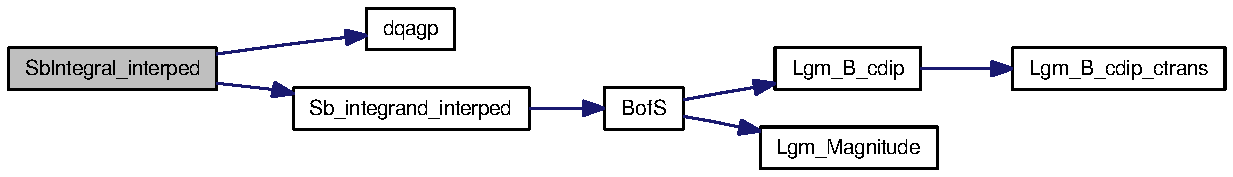
\includegraphics[width=314pt]{_sb_integral_8c_d53ba64293ea16f5d1878d483d62fcd4_cgraph}
\end{center}
\end{figure}
\hypertarget{_sb_integral_8c_1828b0051c3925909496a0d956bcaab3}{
\index{SbIntegral.c@{SbIntegral.c}!Sb\_\-integrand\_\-interped@{Sb\_\-integrand\_\-interped}}
\index{Sb\_\-integrand\_\-interped@{Sb\_\-integrand\_\-interped}!SbIntegral.c@{SbIntegral.c}}
\subsubsection[{Sb\_\-integrand\_\-interped}]{\setlength{\rightskip}{0pt plus 5cm}double Sb\_\-integrand\_\-interped (double {\em s}, \/  {\bf \_\-qpInfo} $\ast$ {\em qpInfo})}}
\label{_sb_integral_8c_1828b0051c3925909496a0d956bcaab3}




Definition at line 154 of file SbIntegral.c.

Here is the call graph for this function:\nopagebreak
\begin{figure}[H]
\begin{center}
\leavevmode
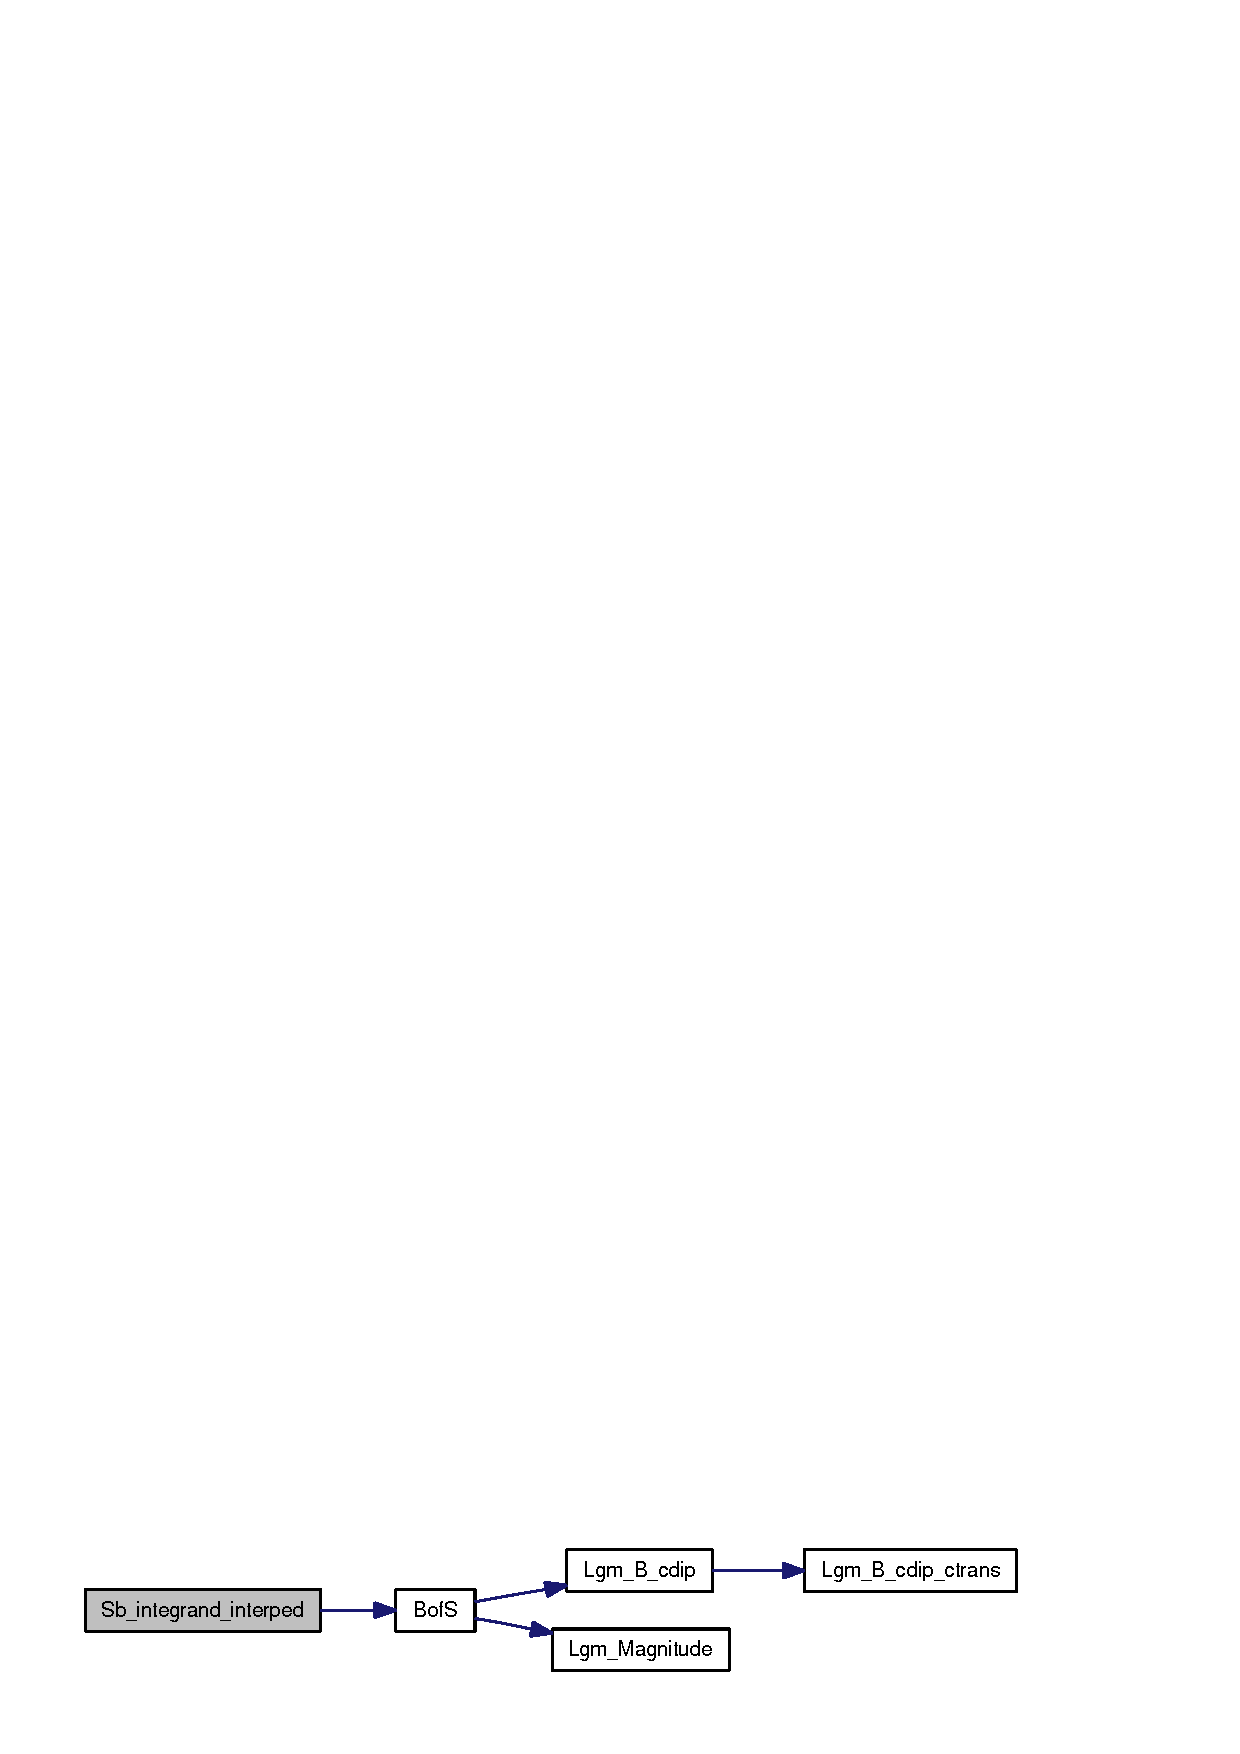
\includegraphics[width=246pt]{_sb_integral_8c_1828b0051c3925909496a0d956bcaab3_cgraph}
\end{center}
\end{figure}


Here is the caller graph for this function:\nopagebreak
\begin{figure}[H]
\begin{center}
\leavevmode
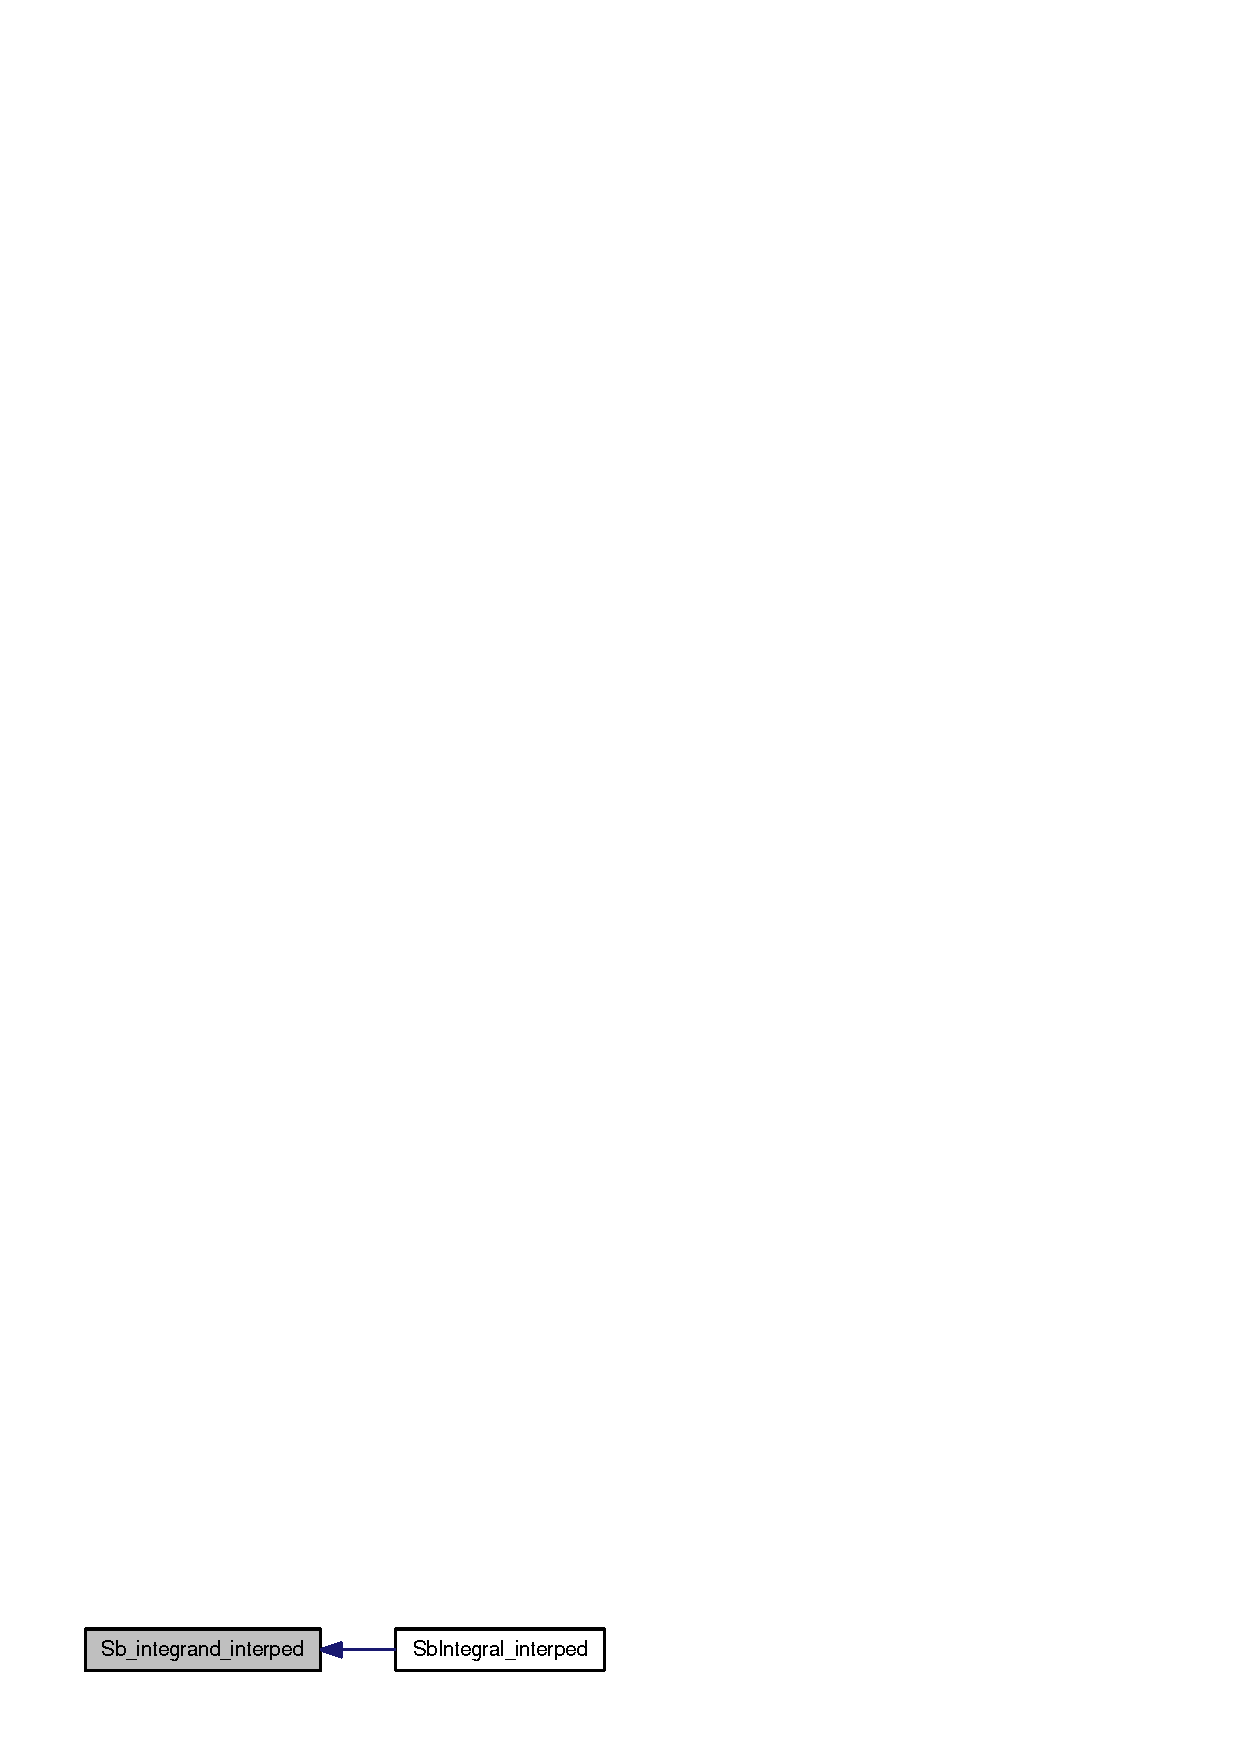
\includegraphics[width=147pt]{_sb_integral_8c_1828b0051c3925909496a0d956bcaab3_icgraph}
\end{center}
\end{figure}
\hypertarget{_sb_integral_8c_23dd3716fba7aa838e159dbf9f447dd0}{
\index{SbIntegral.c@{SbIntegral.c}!Sb\_\-integrand@{Sb\_\-integrand}}
\index{Sb\_\-integrand@{Sb\_\-integrand}!SbIntegral.c@{SbIntegral.c}}
\subsubsection[{Sb\_\-integrand}]{\setlength{\rightskip}{0pt plus 5cm}double Sb\_\-integrand (double {\em s}, \/  {\bf \_\-qpInfo} $\ast$ {\em qpInfo})}}
\label{_sb_integral_8c_23dd3716fba7aa838e159dbf9f447dd0}




Definition at line 174 of file SbIntegral.c.

Here is the call graph for this function:\nopagebreak
\begin{figure}[H]
\begin{center}
\leavevmode
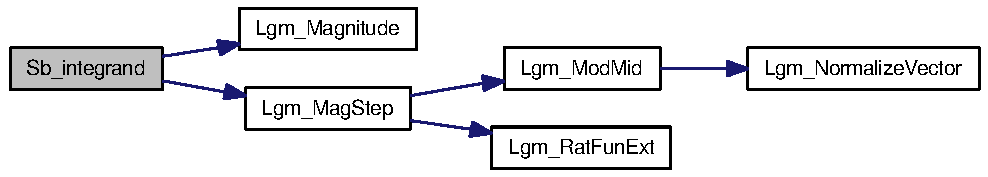
\includegraphics[width=255pt]{_sb_integral_8c_23dd3716fba7aa838e159dbf9f447dd0_cgraph}
\end{center}
\end{figure}


Here is the caller graph for this function:\nopagebreak
\begin{figure}[H]
\begin{center}
\leavevmode
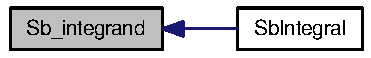
\includegraphics[width=107pt]{_sb_integral_8c_23dd3716fba7aa838e159dbf9f447dd0_icgraph}
\end{center}
\end{figure}
